\section{Results}
\label{sec:results}

Our main result is the comparison of compiled circuit sizes and depths between 
SK and KSV (that is, \emph{quantum resources} at runtime),
and as a secondary result, the comparison of storage requirements (either
classical or quantum, at any stage).
We should note that this comparison cannot be
direct on a per-gate basis for the input circuit $C$ for two reasons.
First, there is a difference between quantum resources needed for a fixed
preprocessing stage, independent of the input circuit $C$. Second there is a
difference between storage requirements for the classical preprocessing stage
or the quantum runtime stage.

%%%%%%%%%%%%%%%%%%%%%%%%%%%%%%%%%%%%%%%%%%%%%%%%%%%%%%%%%%%%%%%%%%%%%%%%%%%%%%%
\subsection{Circuit Size and Depth}
\label{subsec:results-size-depth}

For the fixed quantum preprocessing stage,
KSV expends great effort in creating an initial state
$\ket{\psi_{n,1}}$, which is independent of the input circuit size $S$ or
input circuit depth $D$.
This only has to be done once at the beginning and can
be amortized across all input gates. SK has no such quantum preprocessing
requirements.
Therefore, the correct comparison between
SK and KSV is in terms of their compiled output circuit $C'$ amortized over
the input circuit $C$, for each of the following parameters:
circuit size overhead $S'/S$,
circuit depth overhead $D'/D$,
and circuit width overhead $W'/W$.

The amortized compiled circuit overheads for size and depth are plotted in
Figures \ref{fig:size} and
\ref{fig:depth}, respectively.

\begin{center}
\begin{figure}[h!]
\label{fig:depth}
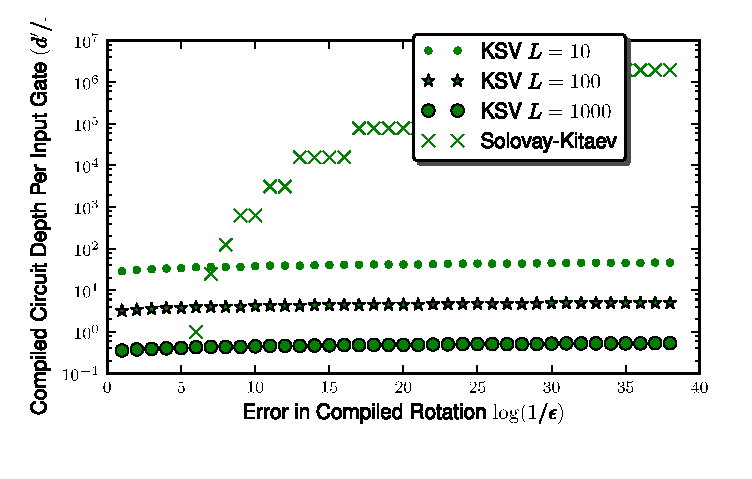
\includegraphics[width=3in]{figures/ksv-depth.eps}
\caption{Compiled circuit depth}
\label{fig:depth}
\end{figure}
\end{center}

\begin{center}
\begin{figure}[h!]
\label{fig:size}
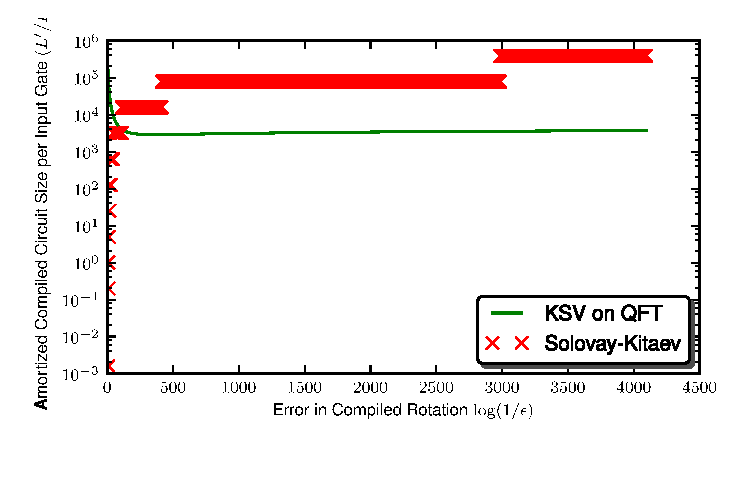
\includegraphics[width=3in]{figures/ksv-size.eps}
\caption{Compiled circuit size}
\label{fig:size}
\end{figure}
\end{center}

The discrete steps in SK's circuit size and depth are due
to the levels of recursion, which are conservatively chosen to meet
the desired precision. The initial step reflects the fact that even
before successive approximation, our initial generated sequences
(basic approximations in Section \ref{sec:sk-algo}) already meet large
desired precisions. As expected, KSV's depth compares very
favorably with Solovay-Kitaev.
The graphs are roughly linear in a log-log plot, with a non-linearity
for low precisions due to irregularities in the adder circuits for small
$n$.

Furthermore, we 

%%%%%%%%%%%%%%%%%%%%%%%%%%%%%%%%%%%%%%%%%%%%%%%%%%%%%%%%%%%%%%%%%%%%%%%%%%%%%%%
\subsection{Circuit Width and Classical Storage}
\label{subsec:results-width}

For the storage requirements, there is no direct comparison possible.
SK has a substantial classical storage requirement
at compile-time which is the dominant resource and is exponential with
the dimension $d$ of a quantum system of $d=2^n$ qubits.
The classical preprocessing time is
also intractable, but for most modern digital computers, storage space is the
bottleneck which is reached first, as shown in Figure \ref{fig:sk-space}.
SK uses no ancillae, so its circuit width overhead $W/W'$ would simply be
a constant 1.

%%%%%%%%%%%%%%%%%%%%%%%%%%%%%%%%%%%%%%%%%%%%%%%%%%%%%%%%%%%%%%%%%%%%%%%%%%%%%%%
%%%%%%%%%%%%%%%%%%%%%%%%%%%%%%%%%%%%%%%%%%%%%%%%%%%%%%%%%%%%%%%%%%%%%%%%%%%%%%%
% Make graph for sk-space.eps here using data on school macbook

%\begin{center}
%\begin{figure}[h!]
%\label{fig:sk-space}
%\includegraphics[width=3in]{sk-space.eps}
%\caption{SK classical preprocessing storage}
%\end{figure}
%\end{center}

On the other hand, KSV has no classical preprocessing stage, and its classical
storage needed for the side-processing in parallelized phase estimation is
efficient (linear in $n$). However, its circuit width overhead is

%%%%%%%%%%%%%%%%%%%%%%%%%%%%%%%%%%%%%%%%%%%%%%%%%%%%%%%%%%%%%%%%%%%%%%%%%%%%%%%
%%%%%%%%%%%%%%%%%%%%%%%%%%%%%%%%%%%%%%%%%%%%%%%%%%%%%%%%%%%%%%%%%%%%%%%%%%%%%%%
% Need a closed formula for circuit width overhead here, and in the table of
% asymptotic bounds in quals-report-definitions


%%%%%%%%%%%%%%%%%%%%%%%%%%%%%%%%%%%%%%%%%%%%%%%%%%%%%%%%%%%%%%%%%%%%%%%%%%%%%%%
%%%%%%%%%%%%%%%%%%%%%%%%%%%%%%%%%%%%%%%%%%%%%%%%%%%%%%%%%%%%%%%%%%%%%%%%%%%%%%%
% Find a way to make this two column to save vertical space!
% Find a way to make this accept PDF rather than EPS



\begin{center}
\begin{figure}[h!]
\label{fig:many-depth}
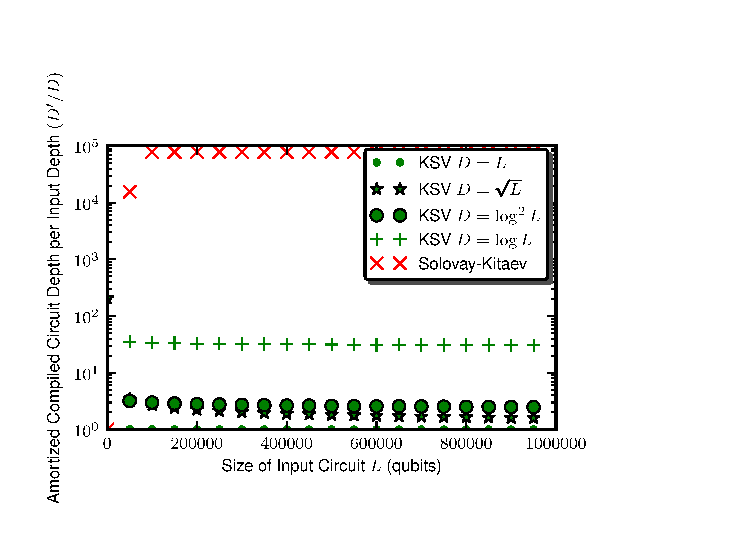
\includegraphics[width=3in]{figures/ksv-many-depths.eps}
\caption{Compiled circuit for various depth/size relationships}
\end{figure}
\end{center}

\begin{center}
\begin{figure}[h!]
\label{fig:one-size}
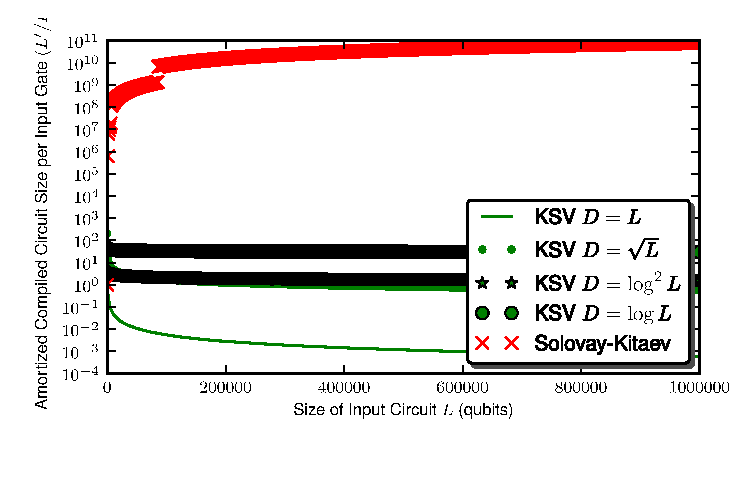
\includegraphics[width=3in]{figures/ksv-one-size.eps}
\caption{Compiled circuit per QFT size}
\end{figure}
\end{center}

The tradeoff between Solovay-Kitaev and Super-Kitaev can most clearly
be seen in the use of space. Solovay-Kitaev uses no ancillae at run-time,
but requires a classical preprocessing step to generate basic
approximations (precompiled sequences from the universal set). Although
we did not generate sequences beyond $l_0 = 9$ for $SU(4)$, the curve
indicates it would soon require terabytes of storage, even if a more
efficient encoding were used (e.g. programming in C instead of Python).
Super-Kitaev, on the other hand, requires no preprocessing space, but
has a (currently intractable) requirement for ancilla qubits are run-time
which tracks the circuit size as $O(n^2 \log n)$.

%%%%%%%%%%%%%%%%%%%%%%%%%%%%%%%%%%%%%%%%%%%%%%%%%%%%%%%%%%%%%%%%%%%%%%%%%%%%%%%
%%%%%%%%%%%%%%%%%%%%%%%%%%%%%%%%%%%%%%%%%%%%%%%%%%%%%%%%%%%%%%%%%%%%%%%%%%%%%%%
% Include graphs here for KSV ancillae usage and SK classical storage
